\documentclass[a4paper, 12pt]{article}
\usepackage[utf8]{inputenc}
\usepackage[english,russian]{babel}
\usepackage[warn]{mathtext}
\usepackage{graphicx}
\usepackage{float}
\usepackage{multirow}
\restylefloat{table}
\usepackage{amsmath}
\usepackage{floatflt}
\usepackage[T2A]{fontenc}
\usepackage[left=20mm, top=20mm, right=20mm, bottom=20mm, footskip=10mm]{geometry}

\tolerance 1414
\hbadness 1414
\emergencystretch 1.5em
\hfuzz 0.3pt        % размер максимального переполнения без warning'a
\widowpenalty=10000 % запрещает одиночную строку абзаца в начале страницы
\vfuzz \hfuzz
\raggedbottom       % если на странице мало содержимого, добавить пустое место в конце, а не в середине страницы



\begin{document}

\begin{titlepage}
	\centering
	\vspace{5cm}
	{\scshape\LARGE московский физико-технический институт (национальный исследовательский университет) \par}
	\vspace{6cm}
	{\scshape\Large Лабораторная работа 5.5 \par}
	{\huge\bfseries Компьютерная $\gamma$-спектроскопия\par}
	\vspace{1cm}
	\vfill
\begin{flushright}
	{\large Б03-104}\par
	\vspace{0.3cm}
	{\LARGE Куланов Александр}
\end{flushright}
	

	\vfill


	Долгопрудный, 2023 г.
\end{titlepage}

\begin{itemize}
	\item \textbf{Цель работы:} Снять и исследовать спектры излучения различных источников, характеризовать различные пики в спектрах радиоактивных веществ.
\end{itemize}

\section{Теоретические сведения}
\textbf{Фотоэффект} - это процесс взаимодействия гамма-кванта с электроном, связанным с атомом, при котором электрону передается вся энергия гамма-кванта. При этом электрону сообщается кинетическая энергия $T_e=E_\gamma-I_i$, где $E_\gamma$ -- энергия гамма-кванта, $I_i$ -- потенциал ионизации $i$-той оболочки атома. Фотоэффект особенно существенен для тяжелых веществ, где он идет с заметной вероятностью даже при высоких энергиях гамма-квантов. В легких веществах фотоэффект становится заметен лишь при относительно небольших энергиях гамма-квантов.  \par
\textbf{Эффект Комптона} - это упругое рассеяние фотона на свободном электроне, сопровождающееся изменением длины волны фотона. Максимальная энергия образующихся комптоновских электронов соответствует рассеянию гамма-квантов на $180^\circ$ и равна
\begin{equation}
E_{\max}=\frac{\eta\omega}{1+\frac{mc^2}{2\eta\omega}}.
\end{equation}
\textbf{Процесс образования электрон-позитронных пар.}
При достаточно высокой энергии гамма-кванта наряду с фотоэффектом и эффектом Комптона может происходить третий вид взаимодействия гамма-квантов с веществом -- образование электрон-позитронных пар. Процесс образования пар не может происходить в пустоте, так как в этом случае не выполняются законы сохранения энергии и импульса. В присутствии ядра или электрона процесс образования пары гамма-квантов возможен, так как можно распределить энергию и импульс гамма-кванта между тремя частицами без противоречия с законами сохранения. При этом если процесс образования пары идет в кулоновском поле ядра или протона, то энергия образующегося ядра отдачи оказывается весьма малой, так что пороговая энергия гамма-кванта $E_0$, необходимая для образования пары, практически совпадает с удвоенной энергией покоя электрона $E_0\cong 2mc^2=1.022$ МэВ.\par
Появившийся в результате процесса образования пар электрон свою энергию на ионизацию среды. Таким образом, вся энергия электрона остается в детекторе. Позитрон будет двигаться до тех пор, пока практически не остановится, а затем аннигилирует с электроном среды, в результате чего появятся два гамма-кванта. Т.е., кинетическая энергия позитрона также останется в детекторе. Далее возможны три варианта развития событий:
\begin{enumerate}
\item оба родившихся гамма-кванта не вылетают из детектора, и тогда вся энергия первичного гамма-кванта останется в детекторе, а в спектре появится пик с $E=E_{\gamma}$;
\item один из родившихся гамма-квантов покидает детектор, и в спектре появляется пик, соответствующий энергии $E=E_{\gamma}-E_0$, где $E_0=mc^2=511$ кэВ;
\item оба родившихся гамма-кванта покидают детектор, и в спектре появляется пик, соотвествующий энергии $E=E_{\gamma}-2E_0$, где $2E_0=2mc^2=1022$ кэВ.
\end{enumerate}
Таким образом, любой спектр, получаемый с помощью гамма-спектрометра, описывается несколькими компонентами, каждая из которых связана с определенным физическим процессом. Как описано выше, основными физическими процессами взаимодействия гамма-квантов с веществом является фотоэффект, эффект Комптона и образование электрон-позитронных пар, и каждый из них вносит свой вклад в образование спектра. Помимо этих процессов, добавляется \textit{экспонента}, связанная с наличием фона, \textit{пик характеристического излучения}, возникающий при взаимодействии гамма-квантов с окружающим веществом, а также \textit{пик обратного рассеяния}, образующийся при энергии квантов $E_{\gamma}\gg mc^2/2$ в результате рассеяния гамма-квантов на большие углы на материалах  конструктивных элементов детектора и защиты. Положение пика обратного рассеяния определяется по формуле:
\begin{equation}
E_{\text{обр}}=\frac{E}{1+2E/mc^2},
\label{eq:Ereverse}
\end{equation}
где $E$ -- энергия фотопика.\par

Даже при поглощении частиц с одинаковой энергией амплитуда импульса на выходе фотоприёмника сцинтилляционного детектора меняется от события к событию. Это связано:
\begin{enumerate}
\item со статистическим характером процессов сбора фотонов на фотоприёмнике и последующего усиления,
\item с различной вероятностью доставки фотона к фотоприемнику из разных точек сцинтиллятора,
\item с разбросом высвечиваемого числа фотонов
\end{enumerate}
\par
В результате в набранном спектре линия (которая для идеального детектора представляла бы дельта-функцию) оказывается размытой, её часто описывают гауссианом.\par
Энергетическим разрешением спектрометра называется величина
\begin{equation}
R_i=\frac{\Delta E_i}{E_i},
\end{equation}
где $\Delta E_i$ -- ширина пика полного поглощения, измеренная на половине высоты, $E_i$ -- энергия регистрируемого $\gamma$-излучения. Значение $E_i$ пропорционально среднему числу фотонов $\overline{n_i}$ на выходе ФЭУ, т.е.:
\begin{equation}
E_i=\alpha\overline{n_i}.
\label{eq:4}
\end{equation}
\par
Полуширина пика полного поглощения $\Delta E_i$ пропорциональна среднеквадратичной флуктуации $\overline{\Delta n_i}$. Т.к. $n_i$ является дискретной случайной величиной, которая распределена по закону Пуассона, то $\overline{\Delta n_i}=\sqrt{\overline{n_i}}$ и поэтому
\begin{equation}
\Delta E_i=\alpha\overline{\Delta n_i}=\alpha\sqrt{\overline{n_i}}.
\label{eq:5}
\end{equation}
\par
Получаем, что
\begin{equation}
R_i=\frac{\Delta E_i}{E_i}=\frac{\text{const}}{\sqrt{E_i}}.
\label{eq:6}
\end{equation}
\par
Поскольку энергетическое разрешение зависит от энергии, его следует указывать для конкретной энергии. Чаще всего разрешение указывают для энергии гамма-линии $^{137}\text{Cs}$ (661.7 кэВ).
\section{Обработка результатов}

Проведем измерения гамма-спектров для $ ^{22}Na, ^{137}Cs, ^{60}Co, ^{241}Am, ^{152}Eu $, а также измерение фона.
	
	Найдем пики полного рассеяния для натрия $ \mathrm{^{22}Na} $ и цезия $ \mathrm{^{137}Cs} $:
	
	\begin{equation}\label{}
	N_{Na\_1} = 749.0 \quad N_{Na\_2} = 1774.2 \quad N_{Cs} = 952.9
	\end{equation}
	
	Известно, что этим пикам соответствуют табличные значения энергии 511, 1275 и 662 кэВ соответственно. Тогда проведем калибровку спектрометра, построив линейную зависимость энергии гамма-кванта от номера канала $ E_j = f(N_j) $. Результат калибровки:


\begin{figure}[H]
	\centering
	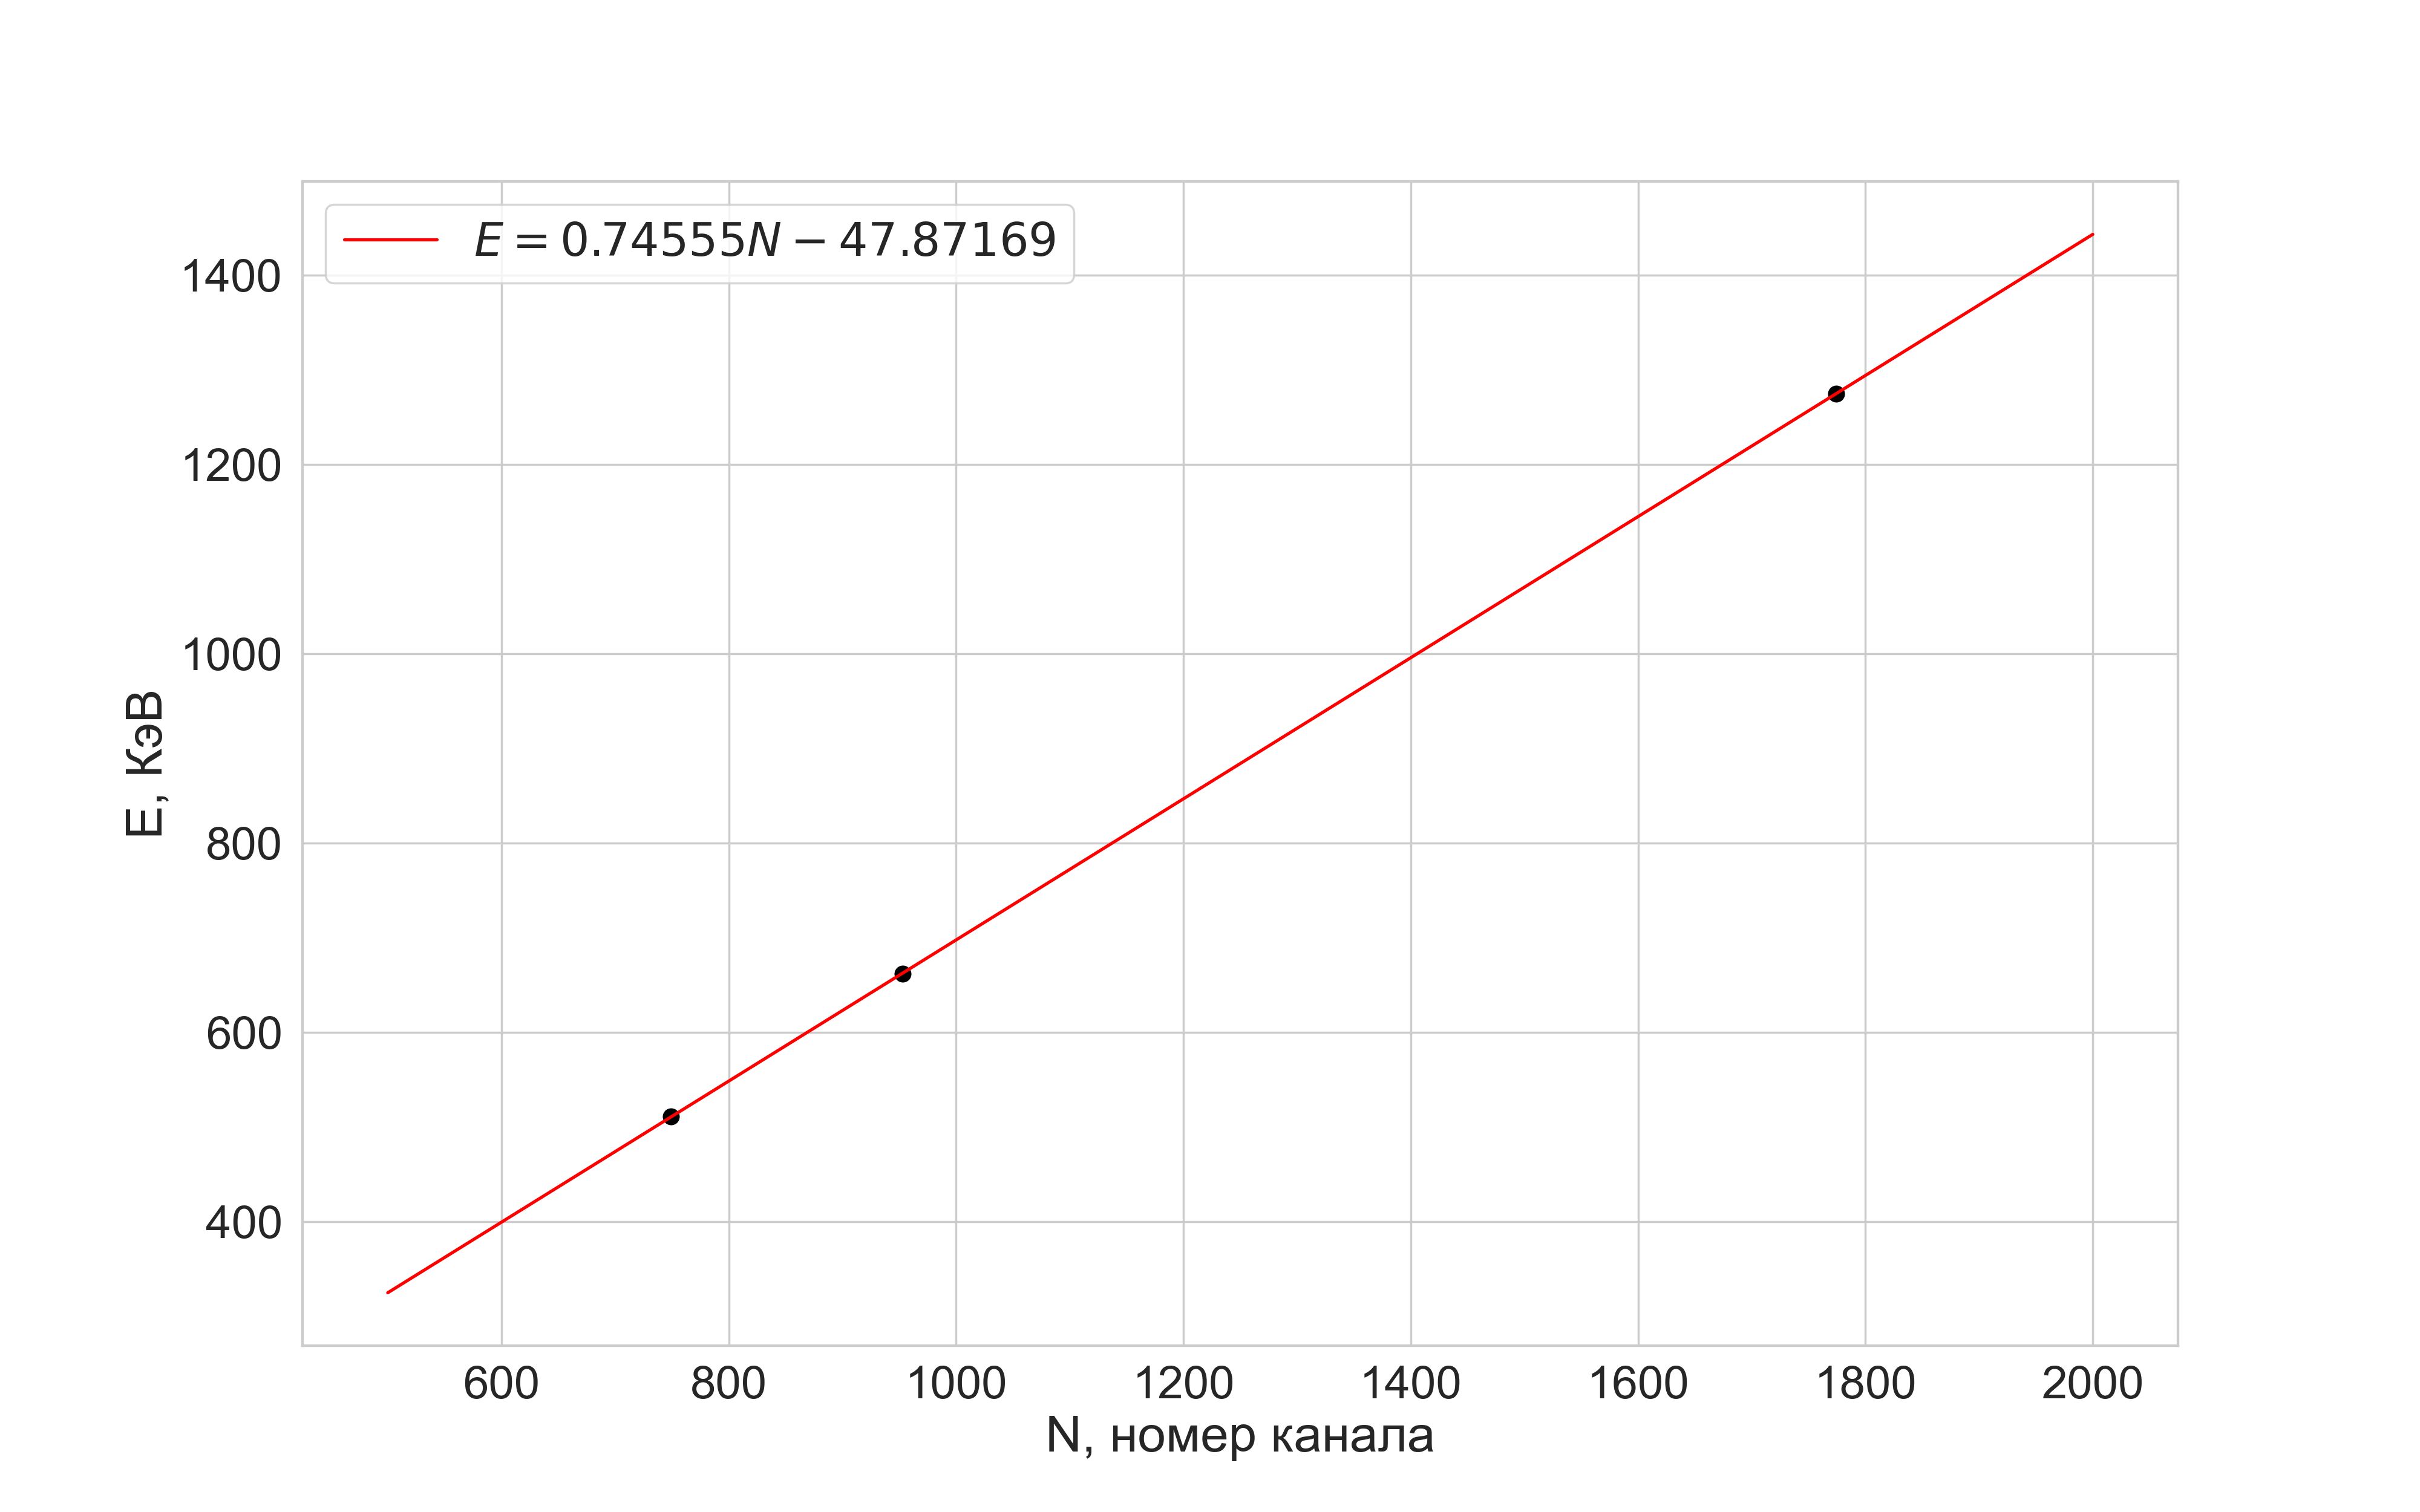
\includegraphics[width=1\textwidth]{plot_calib.png}  \caption{Калибровочный график}
	\label{fig:calib}
\end{figure}

Используя полученную калибровку, найдем положения фотопиков всех элементов

\begin{table}[H]
	\centering
	\begin{tabular}{|c|c|c|c|c|c|c|}
	\hline
	Элемент    & $N_i$ & $\Delta N_i$ & $E_i$, MeV & $\Delta E_i$, MeV & $R_i$ & $E$, MeV \\ \hline
	$^{22}$Na  & 1774  & 69           & 1,275      & 0,051             & 0,04  & 1.274    \\ \hline
	$^{60}$Co  & 1635  & 67           & 1,171      & 0,050             & 0,04  & 1.173    \\ \hline
	$^{60}$Co  & 1854  & 81           & 1,334      & 0,060             & 0,05  & 1.332    \\ \hline
	$^{137}$Cs & 953   & 62           & 0,663      & 0,046             & 0,07  & 0.662    \\ \hline
	$^{241}$Am & 147   & 14           & 0,062      & 0,010             & 0,17  & 0.595    \\ \hline
	$^{152}$Eu & 232   & 16           & 0,125      & 0,012             & 0,1   & 0.122    \\ \hline
	$^{152}$Eu & 393   & 31           & 0,245      & 0,023             & 0,09  & 0.245    \\ \hline
	$^{152}$Eu & 525   & 39           & 0,344      & 0,029             & 0,08  & 0.344    \\ \hline
	\end{tabular}
	\end{table}
Как мы видим, данные похожи на истинные. Построим график $R^2(1/E)$, чтобы убедиться в справедливости соотношения (6). Действительно, зависимость похожа на прямую.
\begin{figure}[H]
	\centering
	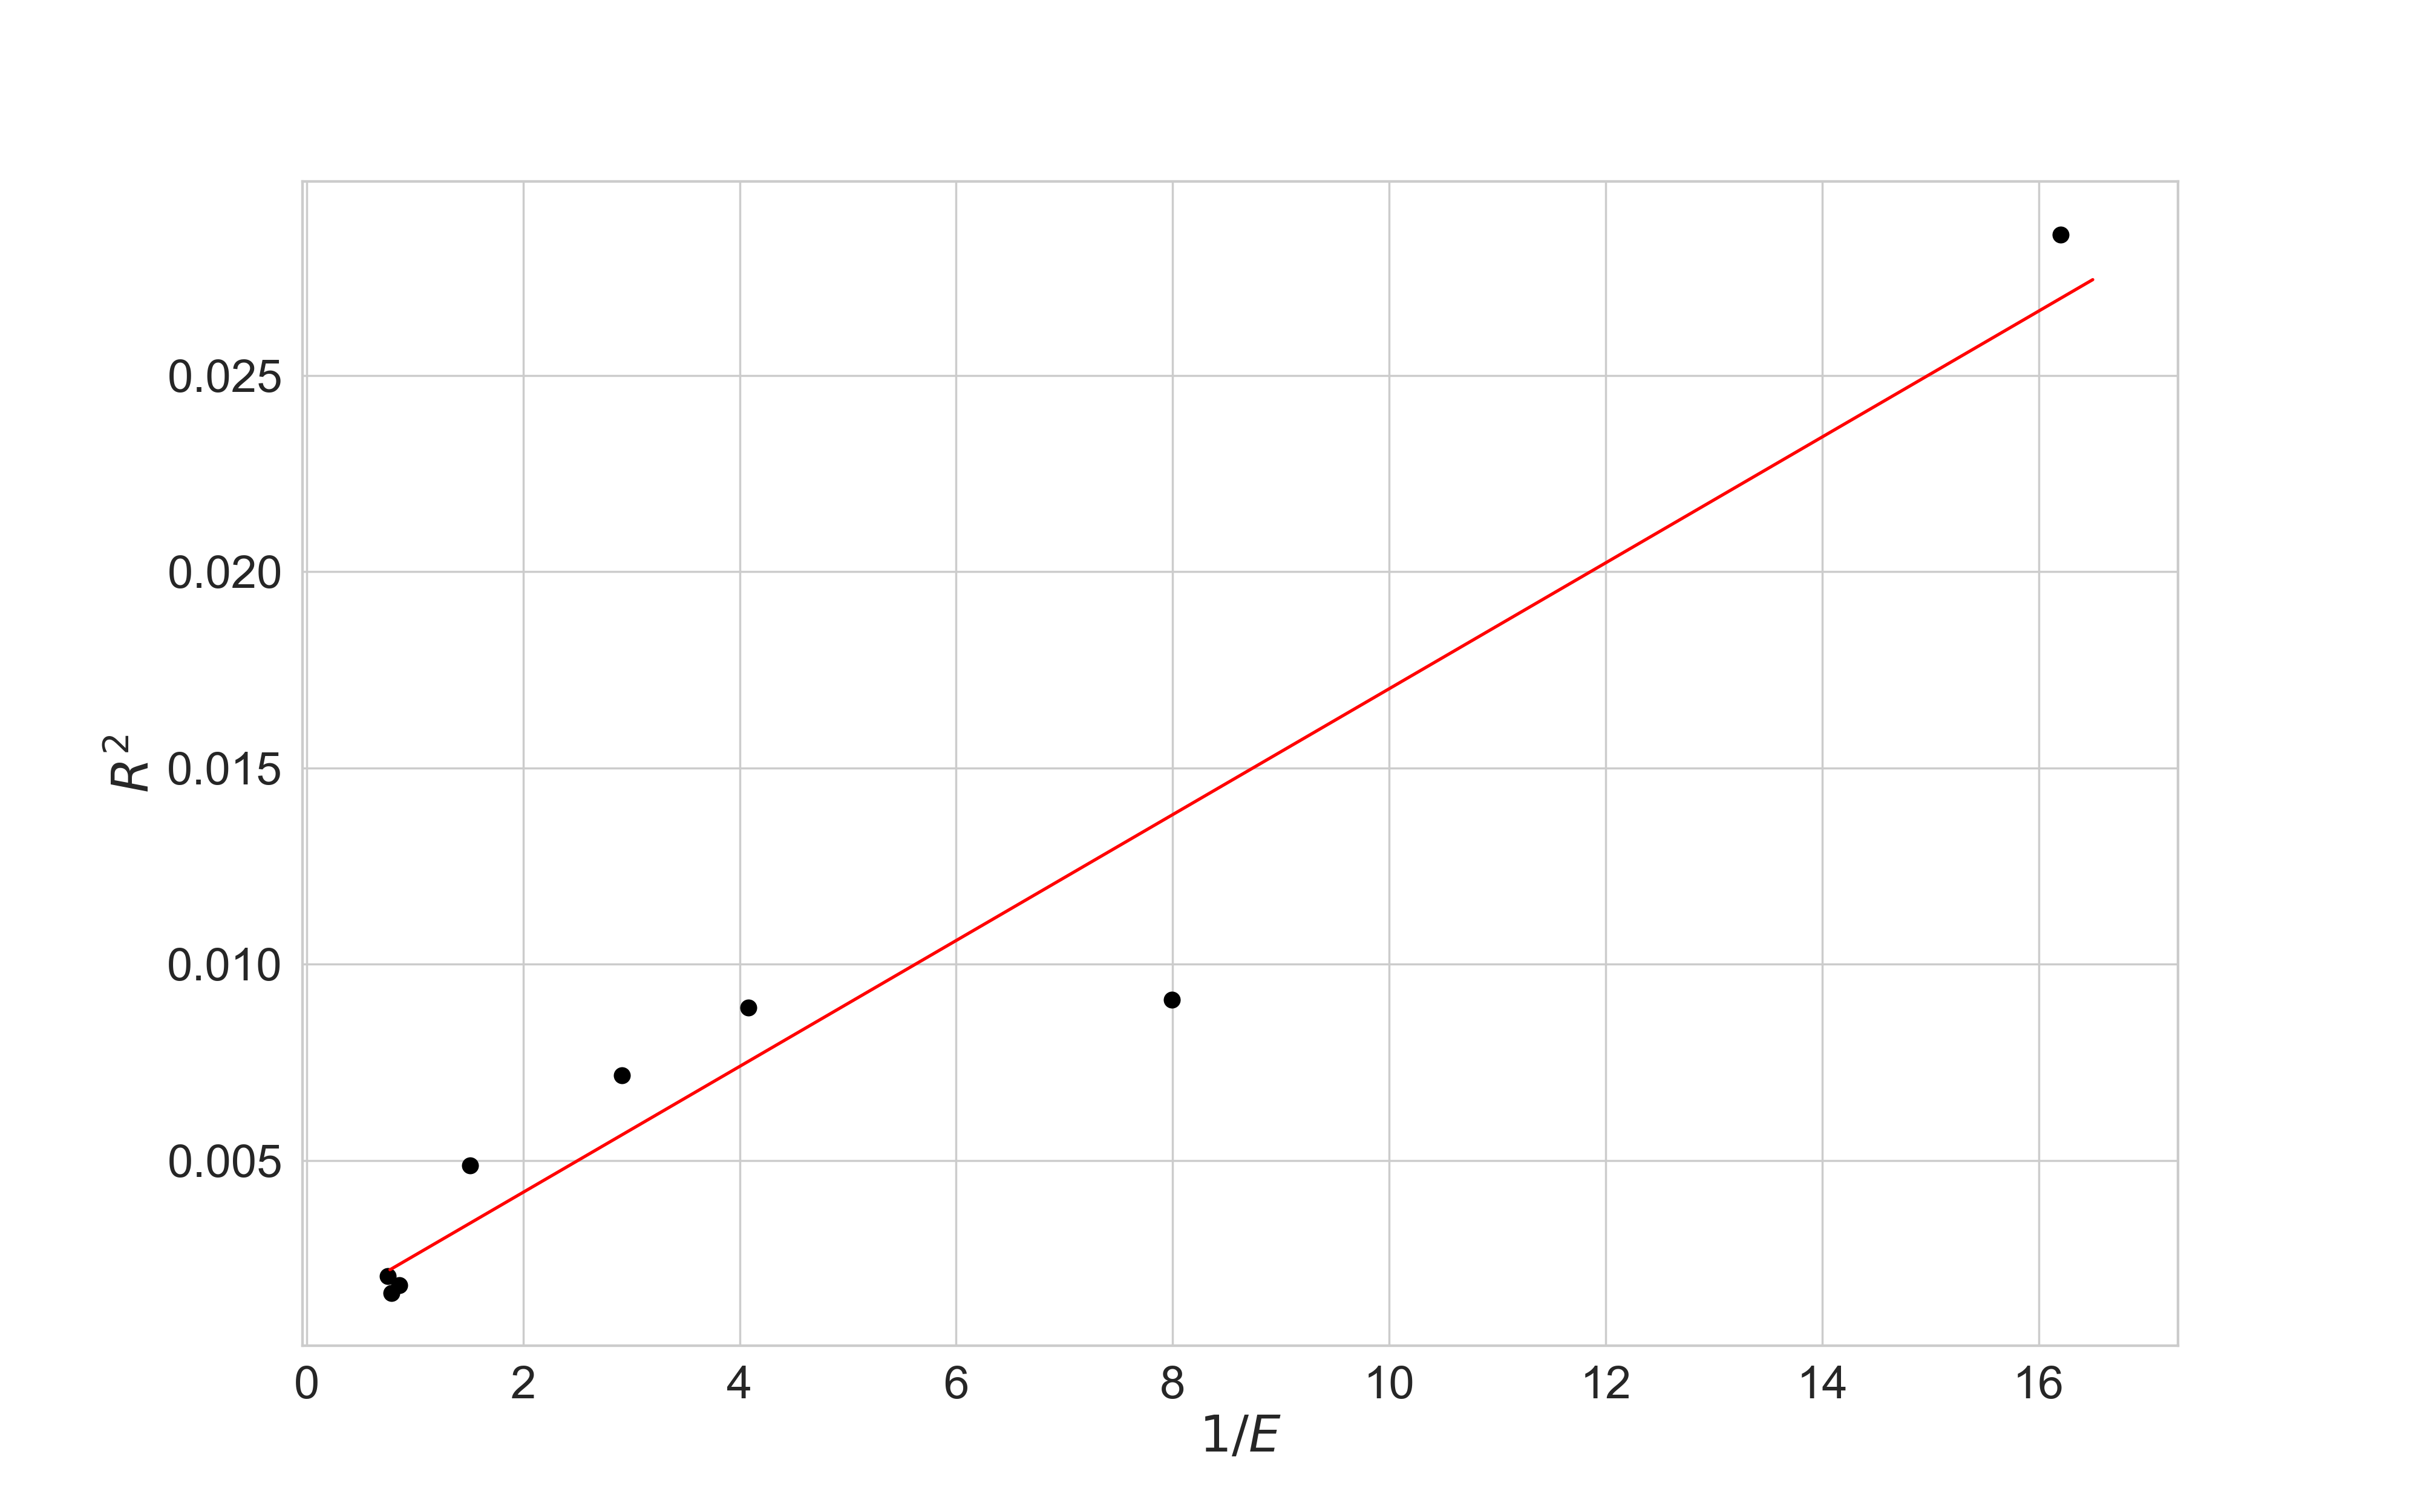
\includegraphics[width=1\textwidth]{plotr2.png}  \caption{График зависимости $R^2(1/E)$}
	\label{fig:plotr2}
\end{figure}
Теперь сравним полученные пики Комптоновского рассеяния с теоретическими значения:

\begin{table}[H]
	\centering
	\begin{tabular}{|c|c|c|c|}
	\hline
	Образец                      & $ N_i $ & $ E_\text{экс}, $ кэВ & $ E_\text{теор}, $ кэВ \\ \hline
	 $ \mathrm{^{137}Cs} $  & 707     & 479,2                & 477.2                  \\ \hline
	$ \mathrm{^{60}Co} $ & 1363    & 968,3                & 960.9                  \\ \hline
	\end{tabular}
	\end{table}
По спектру, например, Натрия, определим пик излучения свинца (самый левый пик на спектре). Он соотвествует каналу с номером 169, или энергии 78 КэВ.
\section{Выводы}
В ходе работы после калибровки прибора были сняты спектры образцов $^{22}$Na,  $^{60}$Cо,  $^{137}$Cs, $^{241}$Am, $^{152}$Eu. В спектрах были исследованы пики, соответствующие следующим взаимодействиям гамма-квантов с веществом:
\begin{itemize}
    \item фотоэффект (пики полного поглощения)
    \item эффект Комптона (характерное распределение энергий в спектре, оканчивающееся комптоновским краем)
    \item аннигиляция позитронов (пик 511 keV в спектре натрия, по которому проводилась калибровка)
\end{itemize}

Все значения энергии, опеределённые по спектрам, практически совпадали с табличными и расчётными. \par

Также была проверена линейная зависимость квадрата спектрального разрешения прибора от величины, обратной энергии полного поглощения.

\end{document}